%\documentclass{article}[14pt]
 \documentclass[10pt]{article}
%\usepackage{multicol, blindtext}

%\documentclass[twocolumn]{article}[14pt]
\usepackage{multicol}
\usepackage{lipsum}

\usepackage{url}

  \usepackage{a4wide}
 \usepackage{pxfonts}  % for the black diamond!

\usepackage{xcolor}
\usepackage{soul}

\newcommand{\hlc}[2][yellow]{{%
    \colorlet{foo}{#1}%F
    \sethlcolor{foo}\hl{#2}}%\prg{m}''
}


\usepackage{rotating}
\usepackage{enumerate}

\usepackage{natbib}
\setlength{\bibsep}{0.0pt}

%\pdfpagewidth=210truemm
%\pdfpageheight=297truemm{0.8cm}

% \addtolength{\topmargin}{-2.4cm}
% \addtolength{\textheight}{3.1cm}
 \headheight     0.0cm
 \errorcontextlines=-1
 \advance\textwidth by 2.1cm
  \advance\oddsidemargin by -1.2cm
 \advance\evensidemargin by -0.6cm
\usepackage[T1]{fontenc}
\usepackage[scaled=1]{helvet}
\renewcommand*\familydefault{\sfdefault}
\usepackage{microtype}


\newcommand{\forget}[1]{} % {{#1}}
\pagestyle{empty}

\newcommand{\etc}{{\it etc.}}
\newcommand{\eg}{{\it e.g.\,}}
\newcommand{\ie}{{\it i.e.\,}}


%\usepackage[usenames]{color}

\usepackage{times}
 \usepackage{latexsym}
\usepackage{listings}
\definecolor{dkgreen}{rgb}{0,0.6,0}
\definecolor{gray}{rgb}{0.5,0.5,0.5}
\definecolor{mauve}{rgb}{0.58,0,0.82}

\lstset{ %
  language=Java,                % the language of the code
  basicstyle=\footnotesize\tt,           % the size of the fonts that are used for the code
  numbers=left,                   % where to put the line-numbers
  numberstyle=\tiny\color{dkgreen},  % the style that is used for the line-numbers
  stepnumber=1,                   % the step between two line-numbers. If it's 1, each line
                                  % will be numbered
  numbersep=5pt,                  % how far the line-numbers are from the code
  backgroundcolor=\color{white},      % choose the background color. You must add \usepackage{color}
  showspaces=false,               % show spaces adding particular underscores
  showstringspaces=false,         % underline spaces within strings
  showtabs=false,                 % show tabs within strings adding particular underscores
  frame=single,                   % adds a frame around the code
  rulecolor=\color{black},        % if not set, the frame-color may be changed on line-breaks within not-black text (e.g. commens (green here))
  tabsize=2,                      % sets default tabsize to 2 spaces
  captionpos=b,                   % sets the caption-position to bottom
  breaklines=true,                % sets automatic line breaking
  breakatwhitespace=false,        % sets if automatic breaks should only happen at whitespace
  title=\lstname,                   % show the filename of files included with \lstinputlisting;
                                  % also try caption instead of title
  keywordstyle=\color{blue},          % keyword style
  commentstyle=\color{gray},       % comment style
  stringstyle=\color{mauve},         % string literal style
  escapeinside={\%*}{*)},            % if you want to add LaTeX within your code
  morekeywords={private,public,final,this,throw,new,||,to,def,any}               % if you want to add more keywords to the set
}

\newcommand{\sparagraph}[1]{{\noindent {\bf {#1}}} \noindent} % {{ \vspace{.05in} \noindent {\textit{\textbf{#1:}}}}}
\newcommand{\dparagraph}[1]{{ \vspace{.04in} \noindent {\bf {#1}}} \noindent}
\newcommand{\prg}[1]{{\mbox{{{\tt #1}}}}}%{\textttt {#1}}}
\newcommand{\TODO}[1]{\textcolor{mauve}{*TODO*}\footnote {#1}}


\begin{document}





\title{
Case for MSR PhD Studentship: \\
{\bf {Cloud-First, Secure, Systems Programming through Types}}
 \vspace{-0.3cm}
 }


\author{
  \small{Professor Sophia Drossopoulou, Imperial College London, UK}
}

 \date{     }

\newcommand{\Deliverable}[1]{\vspace{.06in} {\noindent {\em{Deliverable:\ }} #1 \hfill  $\square$}}




\maketitle



\dparagraph{Abstract}

\noindent
We want to  design and leverage type systems so as to develop a secure systems programming language, which will support cloud-first programming and rack-scale computation.
%We will leverage the
%Ttype system  will deliver safety as well as performance.
\vspace{.07in}
\begin{itemize}
\item
%\noindent
By {\em cloud-first} programming we mean that it will support concurrency as well as seamless distribution. Thus, programs written in this language could run in one node  or on the cloud, without the need for  further adaptation.

\item
%\noindent
By {\em secure}, we mean that the programming language should be  {\em memory-safe}, {\em type-safe},   {\em compartmentalization-safe} as well as  {\em concurrency-safe}.
This security will be enforced by the compiler, and will be guaranteed pervasively: there will be no need to ever break the type system.

\item
%\noindent
By {\em systems programming}, we mean a language which allows us to write  patterns found in operating systems, databases, and cloud-services.
       %, such as stream-processing, asynchronous programming, and two-phase commit.
       We also mean that the performance should match that of %current systems programming languages, such as
 C/C++.
\end{itemize}
%\vspace{.1in}
%\noindent
%With these aims, we want to target secure rack-scale computation.

\dparagraph{Timeliness}

\noindent
The current ever-accelerating growth of cloud infrastructure development has accentuated the urgent need for  secure and performant cloud services. Such services can  be delivered in the large scale required only if programmers were equipped with the appropriate tools. The starting point for such tools is an appropriate  programming language.

While there is a plethora of new programming languages, none sufficiently fits the remit of security and performance: Rust is performant, but requires programmers to either break the type system or rely on difficult-to-prove libraries \cite{rustBelt}, and does not guarantee safe concurrency. Go is type-safe and performant, but does not guarantee safe concurrency either \cite{goRaces}. C and C++ are very performant, but are not type-safe nor concurrency-safe.  C\# offers performance,  type-safety, and   supports formal reasoning \cite{specSharp}, but does not guarantee safe concurrency. Javascript and and its type-safe version Typescript are prevalent, but neither performant nor concurrency-safe. None of these languages address compartmentalization-safety \cite{Saltzer74,dennis:semantics}.

On the other hand, recent developments have shown how type systems can be leveraged to achieve safety as well as performance \cite{snowflake,sylvanPhD}. These works combine  clever algorithms and type systems to deliver performance and security at all levels of abstraction.

We want to build on these ideas and improve on performance and address patterns found in data bases and operating systems. If successful, we will have provided to Microsoft an essential ingredient in the quest for the delivery of safe and  performant cloud services. The proposed research fits well with Microsoft's remit of Confidential Computing, and this proposal is the outcome of discussions with Sylvan Clebsch, David Chisnall, Matthew Parkinson, Juliana Franco and Manuel Costa.

\section{Researchers' Background}

Imperial College London is a one-of-a-kind institution in the UK, focusing solely on science, engineering, medicine and business. It ranked ranked 8th globally and first in London in the QS World University Rankings, as well as 9th in the THE World University Rankings. The Department of Computing has 600 undergraduate and 200 postgraduate students, 60 academics, 15 Postdoc Teaching Fellows, 100 Postdoc RAS, and 200 PhD students. It     ranked 2nd in the UK in the UK Universities Subject Times ranking. It has  strong research groups working on Programming Languages, Software Engineering, Program Analysis and Verification, and Systems.

\subsection{Primary Supervisor at Imperial}

Sophia Drossopoulou is Professor of Programming Languages at the Department of Computing. Her research experience spans Programming Language Design and Implementation, Reasoning about Programs, and Robust Smart Contracts. Among other things, together with Susan Eisenbach, she was the first to develop a model for a large subset of Java; together with Dezani, Damiani  and Giannini, she invented object reclassification -- later adopted under the name of "type-state" \cite{drossopoulou2001fickle}; with Anderson, she was first to propose the migration from untyped to typed  programs \cite{babyJ}  -- later adopted as "gradual typing", and again, with Anderson, she was first to work on type inference for Javascript \cite{infJS}; together with Dezani, Yoshida and Mostrous they were first to adapt session types to object-oriented programming \cite{objSess}; she collaborated with Clarke on the foundations of ownership types  the foundations of ownership  types \cite{clarke2002ownership}; she collaborated with Clebsch on the  design of Pony's type system, \cite{agere15-clebcsh} and with Noble, Miller and Murray on holistic specifications for robust smart contracts \cite{holistic}.

She  has published in top-tier conferences such as ECOOP, OOPSLA, AOSD, ESOP and POPL, and has served -- and is serving on the PCs of ECOOP, OOPSLA, AOSD, ESOP, POPL and PLDI. She has given invited talks and tutorials at ESOP, Discotec, PLISS, and Codemesh. She has served as vice-presindent of AITO, and as PC Chair of ECOOP and ESOP. She is currently serving on Agoric's scientific advisory board on the security of smart contracts.

\subsection{Secondary Supervisor at Imperial}

Peter Pietzuch is a Professor of Distributed Systems at Imperial College London. He leads the Large-Scale Distributed Systems (LSDS) group (http://lsds.doc.ic.ac.uk) that conducts research on new abstractions and infrastructures for building scalable, reliable and secure distributed systems, with a particular focus on security and data management challenges. His work bridges the areas of distributed systems, security, networks, and databases.

He has published over seventy articles in highly competitive venues, including USENIX OSDI, USENIX ATC, ACM SoCC, ACM SIGMOD, VLDB, IEEE ICDE, ACM CoNEXT, IEEE ICDCS, ACM CCS, and ACM/USENIX Middleware. He serves on numerous program committees including USENIX ATC, EuroSys, SIGMOD, VLDB, ICDE, ICDCS, SOCC, WWW and Middleware. He is currently the Chair of the ACM European Chapter of SIGOPS (EuroSys), the PC chair for ICDCS 2018, and PC co-chair for Middleware 2017. Before joining Imperial College London, he was a Post-Doctoral Fellow at Harvard University in the systems research group. He holds MA and PhD degrees from the University of Cambridge.


\subsection{Prospective PhD student}

%Given the wide interest in programming languages at our Department,  we are confident that we will be able to attract a capable PhD student. %However,
We have a very strong prospective  PhD student: Paul Li\`etar, who has a lot of experience and strong research interests in programming languages and security.

 Paul  obtained his Baccalaureate from the Lyc�e Pierre Termier in Grenoble with a "mention  tr\`es bien"  and registered at  the Joint Maths and Computing course at Imperial. He graduated with a First in the summer 2017. For his thesis he worked under Drossopoulou's supervision  on the Pony type system: he made incisive proposals for a much simplified model, detected and corrected several errors in the compiler, and proposed new ideas for generics  \cite{paulThesis}. For this work he was   awarded the  Corporate Partnership Programme Award.

He  worked in the winter 2013/14 at DecaWave using embedded bare metal C for ARM Cortex-M3 devices, then in the summer of 2015 at Google London  on certificate transparency on Android, then in the summer 2016 at Google Mountain View investigating the use of Rust to replace  C/C++ code for Android services, and since 2017 at Google Zurich working onAndroid's device integrity solution protecting against automated fraud and abuse.

He is active in the open-source community in general and also   in the Pony community specifically. He has fixed about 16 compiler bugs, and is blogging both tutorial material on program development, and well as advanced proposals on programming language features. He  has obtained an MSR internship in Cambridge under Juliana Franco's supervision starting January 2018. He plans to then pursue a PhD at Imperial College.



\section{Planned Work}

We will address the aims of this project as follows:
\vspace{.06in}

To support {\em seamless distribution}, i.e. that programs should run on one or several nodes without requiring any adaptation, we will follow
 the actor model. This fits well the  asynchronous nature of communication inherent in real world systems as well as in distributed systems.

To support {\em systems programming} we will   extend the actor model so as   to easily express patterns found in operating systems and databases, e.g. two-phase commit and stream processing. We will integrate synchronization primitives which fit well the actor model, such as joins and multi-cast, and will further enrich it with novel notions of synchronized collaboration.
 
To make our language {\em concurrency-safe}, we will  support concepts of isolation and immutability: sharing of data is data-race free, if the shared  data is immutable, or if  access to it has been given up before sharing. We will integrate notions of borrowing, and expand notions of regions  so as to enhance expressivity of programs, and efficiency of implementations.

To make our language {\em compartmentalization-safe}, we will  use notions of isolation, immutability and regions. These will offer a natural way of expressing which actors might access (i.e. read or mutate which data), and give strong guarantees when such accesses are forbidden.

To make our language {\em memory-safe},   we will not support  \prg{null} nor pointer arithmetic, and  the runtime will perform appropriate runtime checks such array bounds checks.

To make our language {\em type-safe}, we will develop a type system and prove soundness, data-race freedom and locality.

To make our language {\em performant}, we will  leverage types to enhance the performance of the runtime system; we will support manual as well as automatic garbage collection; we will leverage types to make garbage collection safe and fast; we will use highly optimized algorithms for queue representation and data allocation, and will employ highly optimizing compiler tool-chains.
 % and employ them to make our language {\em concurrency safe}, and have been suggested in  CITE, and also used in CITE. Moreover,  CITE to support faster garbage collection. We will expand the ideas of isolation, so as to support notions of borrowing, and also the new concurrency ideas. Moreover, we will leverage the guarantees from the type system to combine manual with automatic garbage collection. The type system will give guarantees that will make manual garbage collection safe, and will also be used to develop fast, fully concurrent garbage collection (actors collect and execute fully concurrently with one another).

Finally, we will validate our ideas though an implementation and case studies, and through further explorations of the design space.

\vspace{.06in}
\noindent
We break the work into the following five workpackages:

\subsection{WP1: Flexible Concurrency Paradigm}


The actor model \cite{actors,agha1987concurrent} proposes actors as the  primitive  of concurrent computation. Actors may execute
behaviours fully concurrently with one another, during which they may create further actors, change their state, and send messages to other actors.
Compare part (a) from Figure \ref{fig:actors}.
Actors are isolated, in that they may not directly read or write other actors' state.
The inherent asynchroneity and the isolation
allow easier reasoning, and make actors a natural fit for modelling the real world, as well as computer architectures.
The popularity of the actor paradigm has recently been growing \cite{armstrong1993concurrent,armstrong2007history,karmani2009actor,akka,pony,agere15-clebcsh,EncoreSFM}.

In situations where it is natural to use a value which is calculated by a different actor, the paradigm has been extended by the concept of futures, and promises % \TODO{Need to explain more}
\cite{futures}, and future chaining \cite{promisingFutures}. These allow an actor to wait until a certain value has been calculated,
such suspended evaluations to be treated as first class values, and to be chained into a work-flow.


Nevertheless, these solutions are  insufficient when a tighter collaboration between
different actors is necessary. Such situations arise when a protocol  requires several interactions among the participating agents,
 such as in two-phase commit and stream processing - patterns found in systems programming.
We want therefore to take inspiration from the join calculus \cite{join}, and
support behaviours which will start executing only when several different messages have been received, and also behaviours which are executed by taking control of {\em several} actors. This will allow us to see a protocol in its entirety rather than interspersed over several different behaviours. % \TODO{ideally, write an example where we see the merit of this.}
Compare parts (b) and (c) from Figure \ref{fig:actors}.

In this workpackage not only will we propose new concurrency primitives, but will also work on their formal semantics. 
This will give us means to describe the semantics succinctly and unambiguously, and
ensure that the proposed features are simple and composable. Moreover, this way we will avoid
    problems arising when large amounts of systems software has been built on a language without a formal semantics;
     such problems emerged for C \cite{CdeFacto}, and the elusive quest of a model of concurrency in C/C++11 \cite{CEleven}.
  The correct time to formalize a language is {\em before} its wider acceptance, and not decades later.

\newcommand{\AAAA}{} % {{\vspace{-1cm}}} %  \hspace{-0.2cm}}}
\newcommand{\BBBB}  {{\vspace{-1.5cm}}}%  \hspace{-0.2cm}}}
\newcommand{\CCCC} {{\vspace{-1cm}}} %  \hspace{-0.2cm}}}
\newcommand{\includeMyFigure}[1]{{   \includegraphics[trim=50 230 100 180,clip,scale=0.33]{#1}  }}
% \includegraphics[trim=left bottom right top, clip]{file}
%[height=6cm]{#1}  }}
% scale=0.25?=�
% 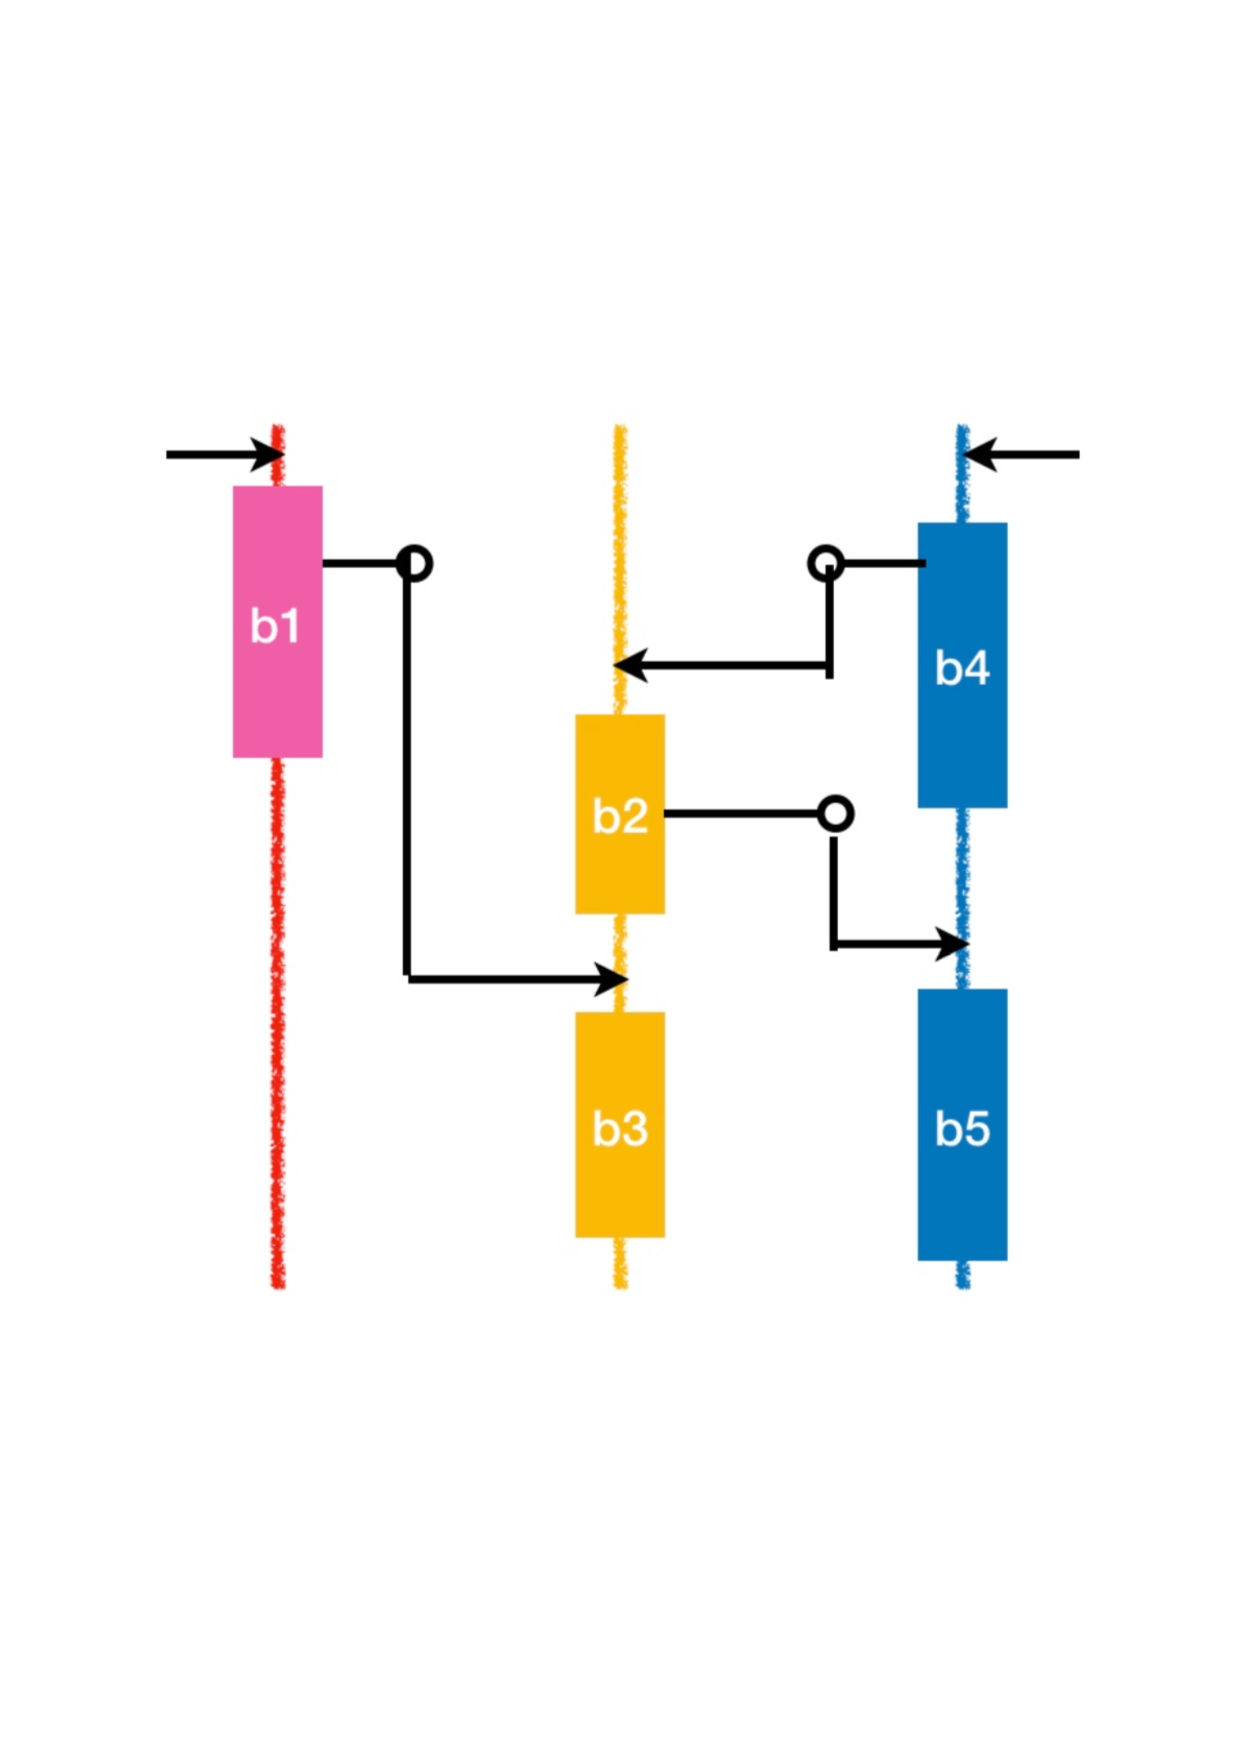
\includegraphics[scale=0.25]{Figs/diagrA}

\begin{figure}[!t]%{r}{75mm}
  \centering
  \begin{tabular}{@{}c|c|c@{}}
  (a) & (b) & (c) \\
    \hline
 {\includeMyFigure{Figs/diagrA}}   &
{\includeMyFigure{Figs/diagrB} }  &
{\includeMyFigure{Figs/diagrC} }
  \\
  \hline
  \end{tabular}
  \caption{ Concurrency. \ \ (a) pure actor paradigm: the pink actor executes behaviour \prg{b1}, which sends a message to the yellow actor; the blue actor executes behaviour \prg{b4}, which sends a message to the yellow actor; the yellow actor takes the blue actor's message from its queue, and executes the appropriate behaviour, etc. The rounded lines indicate sending of messages, and the arrow indicate taking messages from queues; \ \ (b) actors and joins: behavious \prg{b2} can be activated only after receipt of the messages sent by the pink and the blue actor; \ \  (c) actors and collaboration:  while behaviours \prg{b1}, \prg{b2} and \prg{b3} are executed by the corresponding actor separately,  behaviour \prg{b\_collaborate} is a collaboration of all three actors: it can only start when they are all idle, and has access to all these actors' state}
  \label{fig:actors}
\end{figure}






 \Deliverable {An operational semantics for this flexible concurrency paradigm. We will strive to unify the various kinds of synchronization of behaviours and actors, so that futures, promises, joins and collaborations are first class, which can be coordinated through simple temporal ordering relations between them.}



  \subsection{WP2: Flexible, safe, performant isolation}

Isolation   has been used for data-race freedom, for reasoning, and also for automatic garbage collection (GC).
Isolation comes in many slightly different forms, but roughly speaking,
a set of objects is {\em isolated}, if only one actor has access to them, and  this access is dominated by one object. Therefore,
if an actor gives up its access to the dominating object, and passes it to another actor, then the other actor may
modify any of the isolated objects and still be data-race free
\cite{srinivasan2008kilim,agere15-clebcsh,gordon2012uniqueness,haller2010isolated}.


In contrast, Erlang is concurrency-safe, and does not require copying when passing messages, 
but it precludes passing mutable data in messages. Thus
any  mutation needs to be transformed into a slightly altered copy.
 This programming pattern    is particularly 
expensive and cumbersome
 when several  layers from a network or storage stack concurrently work and modify  different parts of the same data structure \cite{solaris}.

Such a set of isolated objects can be seen as a {\em region} \cite{tofte1997region}, or as a set of objects {\em owned} by the dominating object \cite{Noble98flexiblealias}. Objects' membership to such regions can be denoted and guaranteed
through a protocol whereby   regions are created linearly \cite{linear_regions},  or a protocol ensuring that the dominating object creates the rest
      \cite{ClaPotNobOOPSLA98}, or through dependent types using immutable paths \cite{clarke2002ownership,clarke2013aliasing}.     In Figure \ref{fig:types} (b) there are two regions, one is dark green and the other light green. The yellow actor has access to the former through objects \prg{o3} and \prg{o4} and to the latter through object \prg{o1}.
        When the green actor gives up its references to \prg{o3} and \prg{o4} is is safe to send to the yellow actor any of the objects in the dark green region.



Besides their use for data-race free passing of mutable objects,  regions can also used for GC (which our language will provde  to be only for the objects selected by the programmer, see below): As soon as a region goes out of scope or the dominating object becomes unreachable, the whole region (or the whole set of owned objects) can be deallocated without the need of object-graph traversal \cite{PizloFHV04,grossman2002region,regionInferGC}. In In Figure \ref{fig:types} (c), if \prg{o1} became unreachable, the remaining light green objects could be collected.  These approaches however impose a stronger requirement than what is needed for data-race freedom: While opaque  references (i.e.references used only for identity comparison, but precluding read or write) into such regions/ownership sets do not affect data-race freedom, they would need to be forbidden for such region-based automatic garbage collection.

While automatic garbage collection offers convenience and safety,  it comes with the performance penalty of the need to trace the object graph. The Snowflake project  \cite{snowflake} aims to give the best of both worlds: it offers a safe  {\em integrated approach}, whereby programmers can safely chose for each object whether it will be automatically or manually   collected;  for the latter, it guarantees  use-after-free exceptions.

A new approach to fully concurrent garbage collection of objects and actors has been recently proposed, so that actors may trace/GC concurrently with other actors executing behaviours or tracing/GC-ing,  and also actors may be collected fully concurrently with other actors executing behaviours or tracing/GC-ing, without any synchronization or stop-the-world step \cite{clebsch2013fully,orca}. The approach leverages the type system so as to know an object's representation and so as to avoid data-races between actors. It also uses a per-object reference count scheme which gives upper bounds on the number of actors which may access the current object.

\vspace{.1in}

In this project we want to to allow a more flexible system where several regions may  reside on the stack frame,
       and  regions may be coalesced into one, or  separated into an isolated set. We want to extend these ideas so as to also allow borrowing \cite{boyland2001capabilities,boyland2003checking}, whereby a an object graph may be safely shared across n different actors in a read-only mode, and then these n actors are finished, the sending actor will be able to modify it.
       Thus borrowing will allow us to express programming patterns where problems are distributed to workers in a read-only manner, and are then updated given the workers' responses.

We   want to offer an integrated approach to garbage collection, which  combines manual memory management with automatic garbage collection.

And we want to improve on the ideas from \cite{clebsch2013fully,orca}: % so as to avoid tracing as far as possible.
%: For manually managed objects, deallocation will be safe and under the programmer's control. For the autmatically managed objects, 
 Based on the insight that regions may be mutable or immutable, we can reduce the tracing needed. Mutable regions only allow one unique reference into its constituent objects -- thus, by only keeping track of the number of regions that point into an object, we can significantly reduce the tracing needed. Immutable regions may have any number of references pointing into them, but objects' membership  cannot change, and thus repeated tracing can be avoided. Cycles in the object graphs may make GC incomplete \cite{danThesis}, but these can be   discovered in linear time \cite{tarjan}. 
 % \TODO{What about \prg{tag}? I am unclear, unless we just forbid it in some circumstances}.
Finally, borrowing will allow us to temporarily treat objects as immutable, and thus avoid several identical traces through their structures. 
 
 \Deliverable {New concepts of regions allowing for several reasons residing on the stack and for region merge and split, and  data borrowing. New integrated garbage collection protocol, leveraging on types, region-based GC and reference count and on graph algorithms.}

 

 \subsection{WP3: Type System and Formal Models}

Concurrency-safety of our language will be guaranteed by the type system, which will assign  {\em reference capabilities} (unforgeable tokens of authority \cite{levy:capabilities}) to how an actor may   view  an object. These capabilities determine whether an actor may read, write, send an object, or create an alias of a certain kind. The access from the actor to the object may go through several intermediate objects, i.e. though a path starting from a local variable or an actor field and is followed by a sequence  of field accesses. The type system needs to ensure that whenever an actor has a write capability on an object, any other actor can only see this object in an opaque manner -- ie neither read nor write
        \cite{agere15-clebcsh,gordon2012uniqueness}.
         In Figure \ref{fig:types} (a) only two objects are accessible from both the pink and yellow actor: the pink actor and the yellow actor have a read view on \prg{o3};
          the pink actor actor has a write view on \prg{o5} and the yellow actor has an opaque view on \prg{o5} -- this is situation is concurrency-safe. 



Capabilities also support {\em compartmentalization}: Namely, capabilities are statically assigned to paths, and become weaker as the paths become longer; they reflect that the capabilities of the path is a combination of the capabilities of the field references involved in that path. The special capability \prg{iso} indicates that the holder of this reference holds the unique writeable entry into the data structure under it; thus, only the holder of the reference has the ability to modify the data structure.
The special capability \prg{val} indicates that no actor can modify the data structure of this object, either now or ever in the future.

\begin{figure}[!tb]%{r}{75mm}
  \centering
  \begin{tabular}{@{}c|c|c@{}}
  (a) & (b) & (c) \\
    \hline
 {\includeMyFigure{Figs/diagrD}}   &
{\includeMyFigure{Figs/diagr_before} }  &
{\includeMyFigure{Figs/diagr_after} }
  \\
  \hline
  \end{tabular}
  \caption{Concurrency-safety, Regions and Isolation.\ \  a) Here the pink actor and the yellow actor have a read view on object \prg{o3}; the pink actor has a write view on object \prg{o5} and the yellow actor has an opaque view. Thus, we are concurrency-safe. \ \ b) The dark green objects form one region and the light green object form another region. The dark green region is accessible through two stack-based references. \ \ c)  The pink actor gave up its two stack-based references on the  dark green region; thus the objects are now isolated, and it is safe to pass any object from the dark-green region to the yellow actor.}
  \label{fig:types}
\end{figure}
 


\vspace{.1in}

In this project we will integrate the capabilities approach outlined above \cite{agere15-clebcsh,gordon2012uniqueness}  with borrowing and   the new regions described in WP2. We will also integrate with the new concurrency features to be developed in WP1. We  will not support \prg{null} thus avoiding \prg{null}-pointer exceptions \cite{nullHoare} and will support object initialization \cite{initalization}, thus avoiding ugly programming patterns when creating cyclic structures. We want to develop a natural  approach to generics, taking inspiration from materials and shapes \cite{famiglia}. We also want to improve on compartmentlization, by assigning {\em relative} capabilities, eg. forbidding certain actors from ever obtaining a mutable reference to a certain object.

The type system will be  flexible so as to allow the description of any data structure without the need to ever break the type system or revert to low level representations -- as opposed e.g. to Rust which, in order to describe a mutable cyclic structure,  e.g. a doubly-linked list, needs to revert to unsafe code or Hash Maps or use libraries which were developed using unsafe features \cite{RustUnsafe,rustBelt}. 

 

We want to prove type soundness, which will incorporate concurrency-safety, memory-safety, and locality. By the latter, we mean that the behaviour  of one actor is not affected by any other actors; in that sense, a behaviour is linearizable. Moreover, we  want to make the system modular: We  will   describe the capabilities and the regions separately from each other, and describe their combination  only in terms of their emergent properties  but not in terms of their precise definitions. This way, we will have greater flexibility and our results will be applicable to a whole family of capability and regions systems.

 We also want to develop a formal model of the integrated garbage collection protocols from WP2. We want to make the model parametric with the underlying type system, as done e.g. in \cite{orca_formal}, again thus allowing for more applicability of the ideas.
 
 Proofs early on in the development cylce are crucial, for all the reasons we already discussed in WP2.

  \Deliverable {A type system with a detailed soundness proof, and a model of the integrated garbage collection with soundness and completeness arguments.}

\subsection{WP4: Implementation}

The implementation of a new programming language is, indeed, a considerable undertaking, but we  plan to
 base our work on an existing, open-source, efficient implementation developed by the supervisor at MSR  \cite{sylvanPhD}.
 The Pony implementation  consists of  fully-fledged runtime,  including a work-stealing scheduler, garbage collector, memory allocator, message queuing, asynchronous I/O, and more, and a an ahead-of-time optimising compiler targeting LLVM.
Initial, small-scale benchmarks indicate performance of the Pony implementation compares very favourably with that of Scala-Akka, Erlang and  also Go \cite{orca}.

In this work-package we rely on input from the MSR partners. Nevertheless, we are in  a good starting position, since Li\`etar and several of Drossopoulou's UG students have already worked on large code bases, and on the Pony compiler.

\Deliverable{A runtime and compiler to support the works from WP1 and WP2}

\subsection{WP5: Evaluation and Extensions}

We want to try out a series of case studies so as to evaluate our design in terms of programmability and performance. We will start with the known benchmark suites in the actor-targeted Savina test suite \cite{imam2014savina}, and will implement some of the examples in the Computer Languages Benchmark game \cite{CLBMG}. We also want to implement some of the more  interesting part of CCBF\cite{coco}. 

If we have time, we want to also   investigate the distributed implementation of our language. We will need to consider problems related to actor and object migration,  and causality of message delivery \cite{causality}. We have experience from an earlier implementation of a distributed actor language \cite{blessing}, and will also collaborate with Blessing who is currently working on his PhD under Drossopoulou's supervision \cite{causality}.

Also if we have time, we will investigate type inference for our capability annotations, and dynamically typed versions of our language.

\Deliverable{Case studies, and critical evaluation of the language}



 \section{Plans and Feasilbility}



We will start with WP1, and then start  WP2 in month 3, and WP3 in month 6. We plan to have completed the first round of the language design by month 24. We want to start on the implementation in month 14, and hope that some undergraduate students will already have worked on aspects of the garbage collection. We plan to start on case studies (WP5) in month 10, revisit more of them in month 24, and revisit the language design in month 30.


\begin{center} 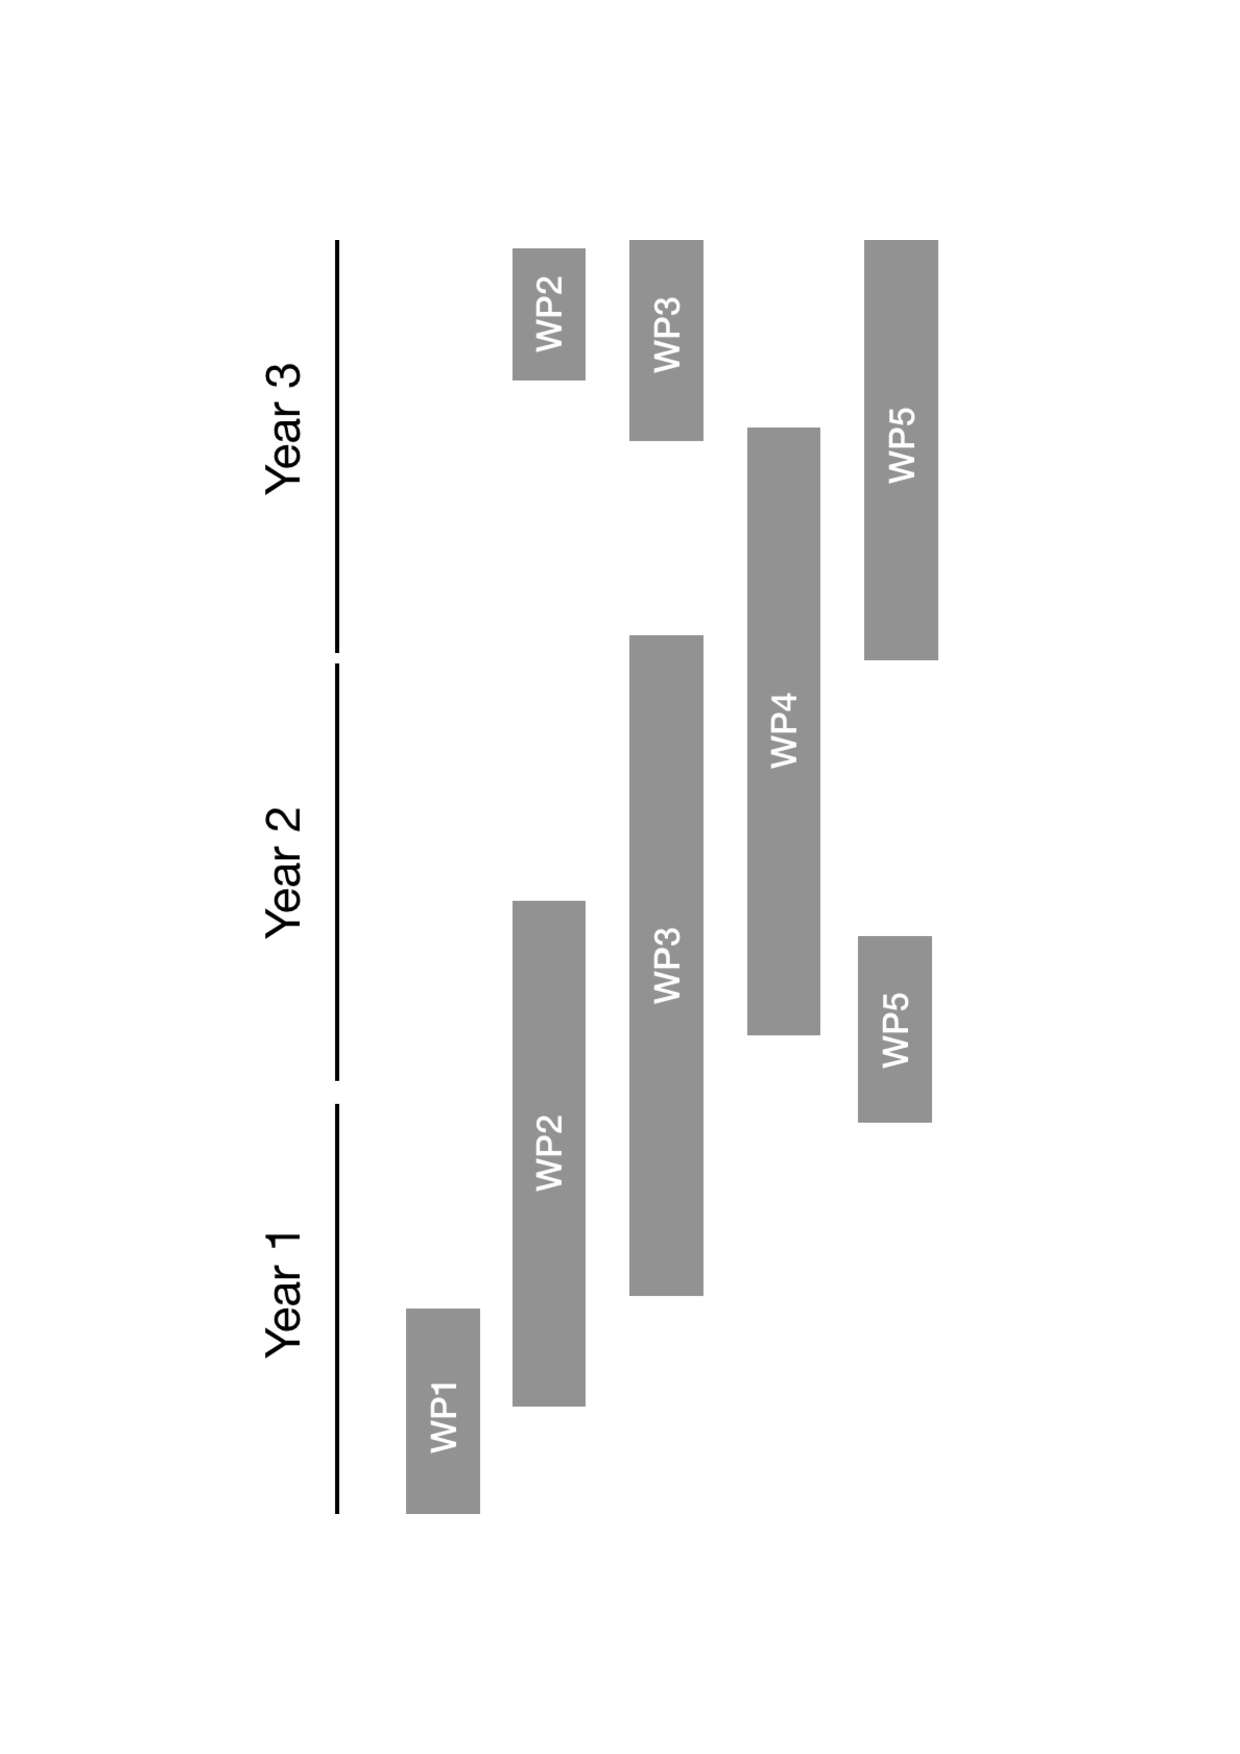
\includegraphics[angle=270,origin=c,scale=0.46,trim=100 100 150 100,clip]{Figs/work}\end{center}
 % top left bottom right

 \vspace{-0.8in}
 This is an ambitious planned work  but we believe that we can deliver most of it, because of our prior work  and our prior collaboration.

Our team has wide experience in programming language design and implementation, and of the Pony implementation which we will be using for our own implementation. Besides her work on actors, Drossopoulou has worked on ownership types  which are related to regions \cite{clarke2002ownership,cameron2007multiple},  on chorded languages which are related to joins \cite{school}, and on traits \cite{smith2005chai}.
The MSR supervisors are world-leaders in the design and implementation of programming languages, security and confidentiality. Also, a large part of this project will build on Clebsch's earlier work \cite{sylvanPhD}.

 % Drossopoulou has received in the past two research gifts from MSR: one to work on Ownership Types, and another to develop
 %material for teaching Dafny. She has visited Judith Bishop in MSR Redmont, and collaborated further with Rustan Leino \cite{}.

Moreover, the MSR and and Imperial supervisor have productively collaborated in the past:
Drosssopoulou was  Clebsch's and  Franco's PhD supervisor at Imperial. She has collaborated with Clebsch
 on the design of the Pony type system \cite{agere15-clebcsh}, and with Franco, Clebsch, and the Uppsalla researchers   on  the evaluation and formalization of the Pony garbage collector \cite{clebsch_drossopoulou_2013,orca,orca_formal}. She has also collaborated with Clebsch and  Slocombe on further improvements of the garbage collector in the presence of immutable objects \cite{danThesis}.
Li\`etar  has already collaborated with Drossopoulou and with Clebsch.
% 
Pietzuch already holds an MSR studentship, collaborating with Clebsch and Costa. 


Moreover, we expect to be able to allocate some of the work to some of our very bright UG and PG students -- indeed, in the past we have been able to develop significant parts of language design and implementation in collaboration with Imperial undergraduate students  \cite{georgeThesis, lukeThesis, danThesis, paulThesis}.

%  \setlength{\itemsep}{0pt} %hack into  bbl file
\bibliographystyle{abbrv}
\bibliography{Case,bibliography}



 % \end{multicols}
\end{document}


